% !TeX program = xelatex
% !TeX encoding = UTF-8
% !TeX TXS-program:compile = txs:///xelatex | txs:///xelatex
\documentclass[aspectratio=169, table, 12pt]{beamer}
% Preamble bersama seluruh slide mata kuliah ini.
% Dipanggil dari slides/sessionXX/sessionXX.tex tepat sesudah baris
% \documentclass[aspectratio=169, table, 12pt]{beamer}
% Paket tambahan yang hanya dibutuhkan satu sesi ditulis di berkas sesi itu.

\usepackage{colortbl}
\usepackage{xcolor}
\usepackage{listings}
\usepackage{tabularx}
\usepackage{booktabs}
\usepackage{tikz}
\usepackage{pgfplots}
\pgfplotsset{compat=1.18}
\usetikzlibrary{arrows.meta, positioning, calc, fit, shapes.geometric,
	shapes.multipart, backgrounds, matrix, chains, trees}

\makeatletter
\def\input@path{{../theme/}}
\makeatother
\graphicspath{{../theme/}{../../figures/}}
\usetheme{Pradita}

\definecolor{praditagreen}{RGB}{37, 113, 71}

% Tema membuat garis tabel berwarna putih. Dikembalikan agar tabel terbaca.
\arrayrulecolor{black}
\setlength{\arrayrulewidth}{0.5pt}

\lstdefinelanguage{yaml}{
	basicstyle=\ttfamily\scriptsize,
	keywordstyle=\color{blue}\bfseries,
	commentstyle=\color{gray}\itshape,
	stringstyle=\color{red},
	showstringspaces=false,
	breaklines=true,
	frame=lines,
	numbers=none,
	backgroundcolor=\color{lightgray!10},
	tabsize=2,
	morecomment=[l]{\#}
}

\lstdefinelanguage{json}{
	basicstyle=\ttfamily\scriptsize,
	stringstyle=\color{red},
	commentstyle=\color{gray},
	breaklines=true,
	showstringspaces=false,
	tabsize=2,
	numbers=none,
	frame=lines,
	backgroundcolor=\color{lightgray!10},
	string=[s]{"}{"}
}

\lstdefinelanguage{bash}{
	keywords={},
	basicstyle=\ttfamily\scriptsize,
	ndkeywords={docker, kubectl, helm, curl, git, terraform},
	ndkeywordstyle=\color{purple}\bfseries,
	sensitive=true,
	commentstyle=\color{gray},
	numbers=none,
	breaklines=true,
	frame=lines,
	backgroundcolor=\color{lightgray!10},
	tabsize=2,
	comment=[l]{\#},
	showstringspaces=false
}

\lstdefinelanguage{http}{
	keywords={GET, POST, PUT, PATCH, DELETE, HEAD, OPTIONS, HTTP},
	basicstyle=\ttfamily\scriptsize,
	keywordstyle=\color{blue}\bfseries,
	sensitive=true,
	numbers=none,
	breaklines=true,
	frame=lines,
	backgroundcolor=\color{lightgray!10},
	tabsize=2,
	showstringspaces=false
}

\subtitle{IT40613 · Digital Platform \& API Economy}
\author{\textbf{Alfa Yohannis}}


\title{\Huge Manajemen Siklus Hidup API\\ \vspace{10pt} dan API Gateway}
\date{Pertemuan 10}

\begin{document}
\frame{\titlepage}

\begin{frame}
  \frametitle{Isi Pertemuan}
  \vspace{14pt}
  \begin{columns}[t]
    \column{0.5\textwidth}
    {\small\tableofcontents[sections={1-5}]}

    \column{0.5\textwidth}
    {\small\tableofcontents[sections={6-10}]}
  \end{columns}
\end{frame}

\begin{frame}{\hfill}
  \centering
  \Huge{\textbf{12 klinik masih di versi lama.\\Ditutup: 720 pemesanan gagal.\\Dibiarkan: Rp45 juta setahun.\\Siapa yang memutuskan?}}
\end{frame}

\section{Tujuan dan Konteks}

\begin{frame}{{\Large Tujuan Pembelajaran}}
  \vspace{10pt}
  \begin{itemize}
    \item Menjelaskan tahap siklus hidup API dan keputusan penting di tiap tahap.
    \item Menjelaskan fungsi \textit{API gateway} dan komponen platform manajemen API.
    \item Membandingkan alternatif platform manajemen API dengan kriteria yang dapat dipertanggungjawabkan.
  \end{itemize}
\end{frame}

\begin{frame}{{\Large Diagram Konsep Bab 10}}
  \centering
  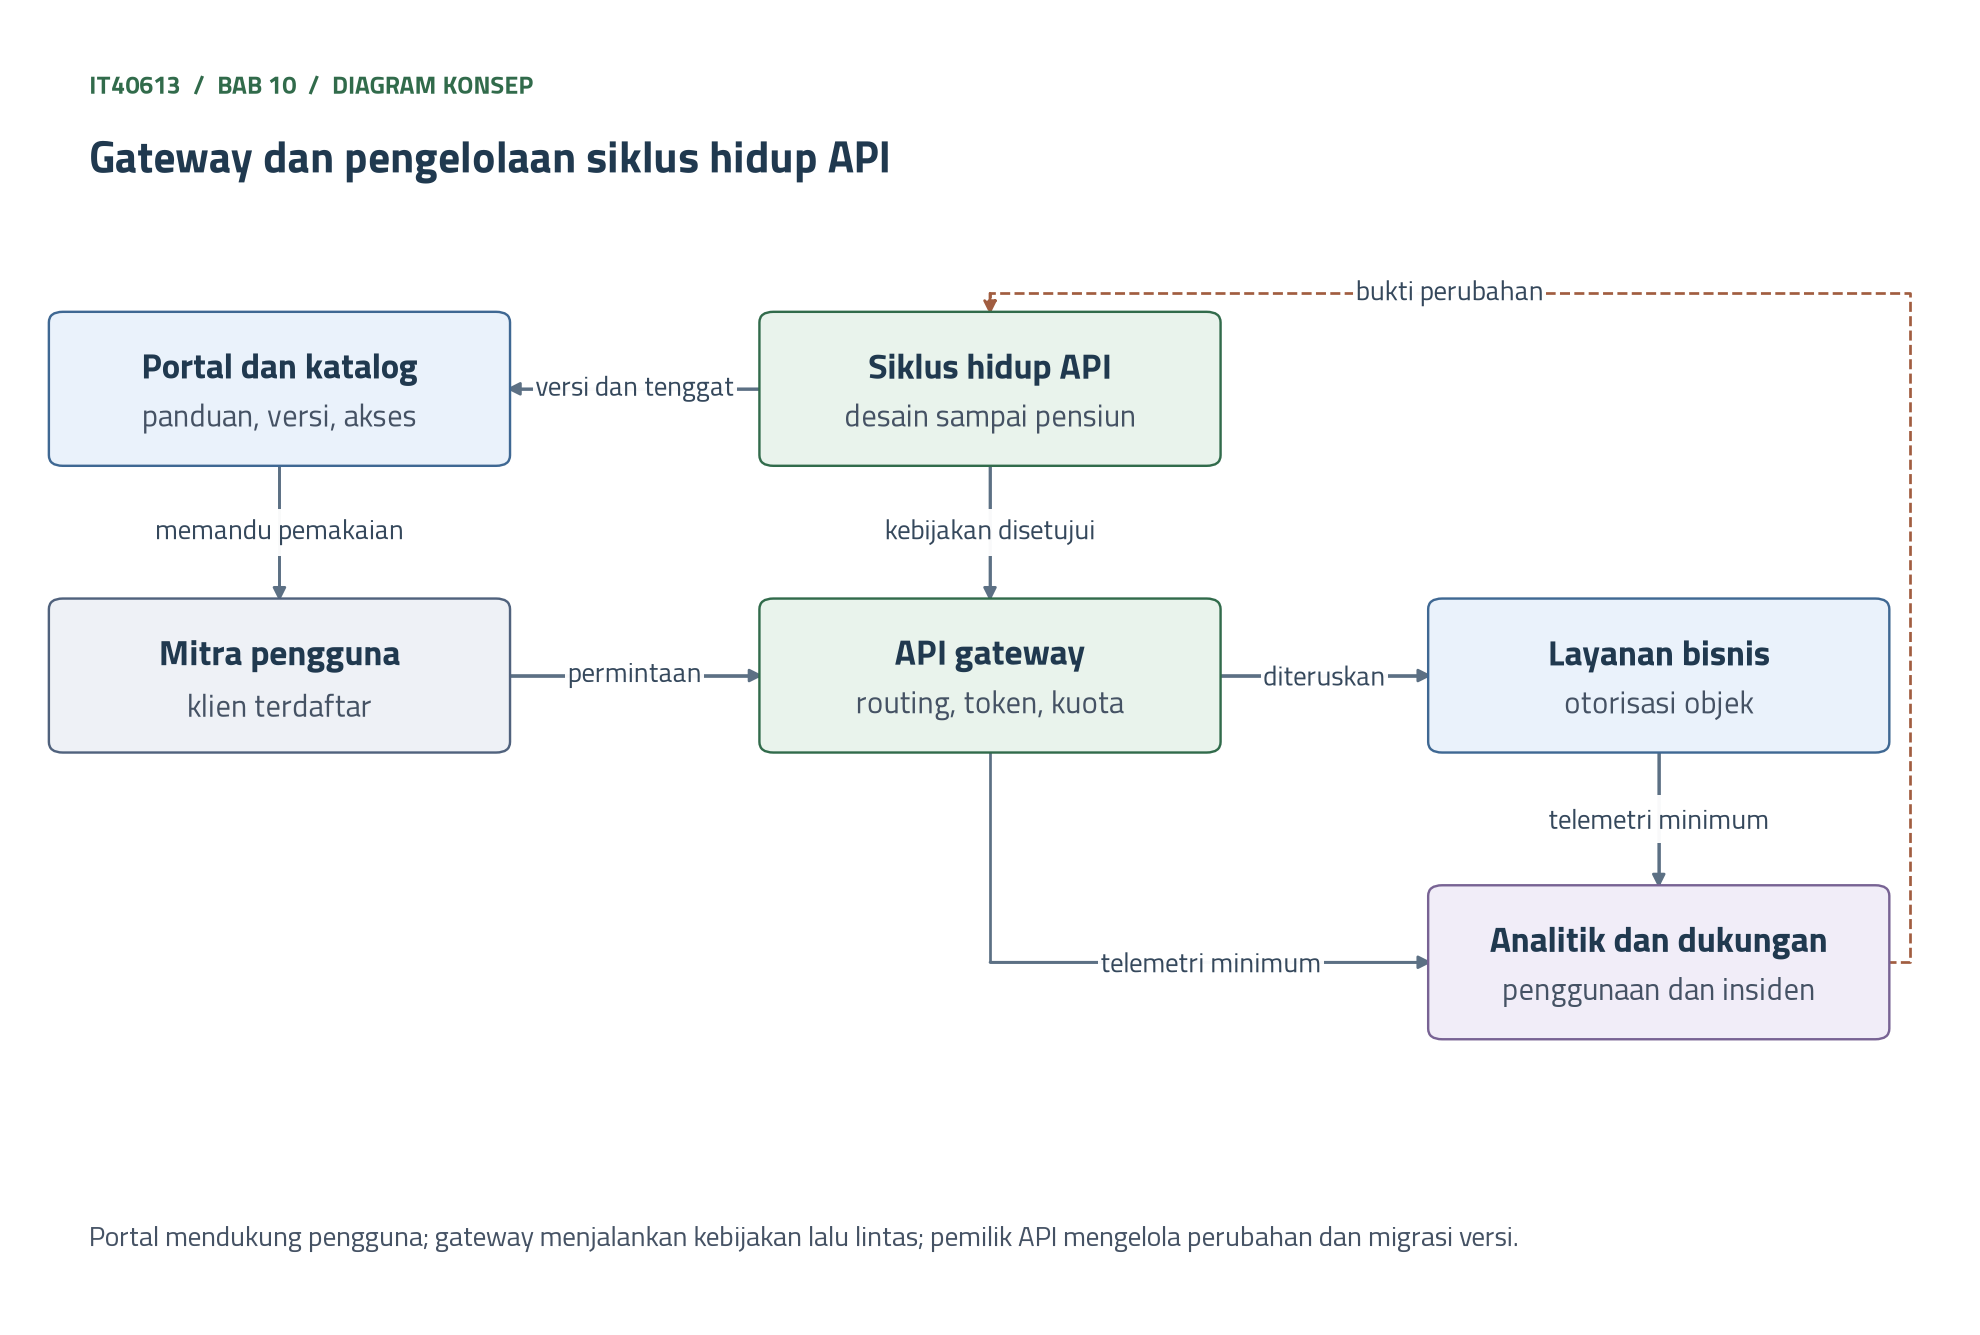
\includegraphics[width=0.96\textwidth,height=0.77\textheight,keepaspectratio]{../../figures/ch10-diagram-konsep.png}
\end{frame}

\begin{frame}{{\Large Masukan dari Bab Sebelumnya}}
  \footnotesize
  \begin{tabularx}{\textwidth}{>{\raggedright\arraybackslash}p{1.3cm} >{\raggedright\arraybackslash}X >{\raggedright\arraybackslash}p{5.0cm}}
    \hline
    \textbf{Asal} & \textbf{Temuan yang dipakai} & \textbf{Kegunaan di sini} \\ \hline
    Bab 4 & Lapisan bersama Rp300 juta per tahun, Rp45 juta per antarmuka & Pagu platform \\ \hline
    Bab 5 & Rantai pemesanan 99,40 persen, 168 gagal per bulan & Dampak \textit{gateway} \\ \hline
    Bab 6 & Register RA-01 sampai RA-07, kuota 300 per hari, 444.000 catatan & Kebijakan di \textit{gateway} \\ \hline
    Bab 8 & 40 klinik, tim 7.680 jam, cadangan 1.080 jam & Kapasitas operasi \\ \hline
    Bab 9 & Kontrak API-01, Two in Production, alamat \texttt{/v2} & Masa transisi \\ \hline
  \end{tabularx}

  \vspace{8pt}
  \small Tarif Rp60.000 per jam, 20 sambungan aktif Rp900 juta per tahun. Vendor Medikara+ butuh 4 bulan.
\end{frame}

\section{Siklus Hidup API}

\begin{frame}{{\Large Lima Tahap Siklus Hidup}}
  \vspace{8pt}
  \begin{itemize}
    \item Rangkaian tahap yang dilalui satu API sejak gagasan sampai dihentikan.
    \item Medjaoui dkk.: \textit{create}, \textit{publish}, \textit{realize}, \textit{maintain}, \textit{retire}.
    \item Bab ini: pembuatan, penerbitan, realisasi nilai, pemeliharaan, pensiun.
    \item Setiap perpindahan memerlukan bukti yang sesuai risikonya.
    \item Status API harus terlihat di katalog.
  \end{itemize}
  \vspace{6pt}
  {\small Analogi: kendaraan dinas tetap membayar pajak sampai surat penghapusannya selesai.}
\end{frame}

\begin{frame}{{\Large Empat Gerbang Bukti}}
  \centering
  \eadiagram{../../figures/ch10-siklus-hidup.tex}
\end{frame}

\begin{frame}{{\Large Keputusan Penting di Tiap Tahap}}
  \footnotesize
  \begin{tabularx}{\textwidth}{>{\raggedright\arraybackslash}p{2.3cm} >{\raggedright\arraybackslash}p{4.2cm} >{\raggedright\arraybackslash}X}
    \hline
    \textbf{Tahap} & \textbf{Keputusan penting} & \textbf{Bukti pada API-01} \\ \hline
    Pembuatan & Layak dibangun, isi kontrak & Kanvas Bab 8, kontrak Bab 9, uji otorisasi objek \\ \hline
    Penerbitan & Siapa boleh memakai, kapan & 5 klinik uji berhasil, dukungan dan rencana cadangan siap \\ \hline
    Realisasi nilai & Apakah janji nilai terbukti & Telepon konfirmasi dari 240 ke 48 per hari \\ \hline
    Pemeliharaan & Perubahan mana dikerjakan & Tiga gerbang Bab 9, 12 usulan dengan kapasitas 6 \\ \hline
    Pensiun & Kapan dihentikan, apa gantinya & Pemakai aktif nol. Pemicu: klinik aktif di bawah 30 \\ \hline
  \end{tabularx}
\end{frame}

\begin{frame}{{\Large Dua Contoh Berangka}}
  \vspace{8pt}
  \begin{itemize}
    \item API-02 tidak terbit hanya karena kode selesai. Misalkan tinjauan 5 orang, 2 jam: Rp600.000.
    \item Satu kredensial bersama bocor: 40 klinik, 2 jam, Rp4,8 juta, atau 8 kali tinjauan.
    \item Misalkan antarmuka yang tidak dipakai dibiarkan 3 tahun: Rp135 juta.
    \item OWASP: penyerang biasanya masuk lewat versi lama tanpa tambalan.
    \item Empat gerbang: Rp2,4 juta per API, atau Rp7,2 juta untuk tiga API.
  \end{itemize}
\end{frame}

\begin{frame}{{\Large Tingkat Kematangan: API-m-FAMM}}
  \scriptsize
  \begin{tabularx}{\textwidth}{>{\raggedright\arraybackslash}p{2.9cm} >{\raggedright\arraybackslash}X >{\raggedright\arraybackslash}p{5.1cm}}
    \hline
    \textbf{Area fokus} & \textbf{Kapabilitas} & \textbf{Keadaan Medikara (pemisalan)} \\ \hline
    \textit{Lifecycle Management} & Versi, pemisahan, pemberitahuan & Belum ada API mitra dan kebijakan versi \\ \hline
    \textit{Security} & Autentikasi, otorisasi, ancaman, enkripsi & Register RA-01 sampai RA-07 sudah ada \\ \hline
    \textit{Performance} & Sumber daya, lalu lintas & Kuota 300 masih rancangan \\ \hline
    \textit{Observability} & Pemantauan, pencatatan, analitik & Catatan rinci 7 hari pada kasus insiden \\ \hline
    \textit{Community} & \textit{Onboarding}, dukungan, dokumentasi & Belum ada portal mitra \\ \hline
    \textit{Commercial} & SLA, monetisasi, akun & Rp3 juta per klinik per bulan masih usulan \\ \hline
  \end{tabularx}

  \vspace{6pt}
  \small 6 area, 20 kapabilitas, 80 praktik. Baca per area, seperti rapor per mata pelajaran. Kematangan bukan jumlah fitur \textit{gateway}.
\end{frame}

\section{Versi dan Deprecation}

\begin{frame}{{\Large Versi dan Deprecation}}
  \vspace{8pt}
  \begin{itemize}
    \item Versi menjelaskan kontrak yang didukung.
    \item \textit{Deprecation}: kontrak tidak lagi dianjurkan dan akan dihentikan.
    \item RFC 9745: perilaku API tidak berubah oleh \textit{deprecation}.
    \item Kebijakan: alasan, jadwal, pengganti, cara menguji, bantuan migrasi.
    \item Versi baru tidak membebaskan penyedia dari komunikasi kepada pemakai lama.
  \end{itemize}
  \vspace{6pt}
  {\small Analogi: nomor telepon layanan lama tetap tersambung selama masa pengalihan.}
\end{frame}

\begin{frame}{{\Large Yang Sering Tertukar: Deprecation dan Sunset}}
  \footnotesize
  \begin{tabularx}{\textwidth}{>{\raggedright\arraybackslash}p{2.1cm} >{\raggedright\arraybackslash}X >{\raggedright\arraybackslash}X >{\raggedright\arraybackslash}p{3.2cm}}
    \hline
    \textbf{Keadaan} & \textbf{Arti} & \textbf{Perilaku versi 1} & \textbf{Tanda} \\ \hline
    Didukung & Kontrak berlaku penuh & Menjawab seperti kontrak & Status di katalog \\ \hline
    \textit{Deprecation} & Tidak dianjurkan, pengganti tersedia & Tetap menjawab, klinik baru tidak diterima & \textit{Header} \texttt{Deprecation}, surel, portal \\ \hline
    \textit{Sunset} & Dihentikan pada waktu yang diumumkan & Sesudahnya menjawab 410 & \textit{Header} \texttt{Sunset}, kode 410 \\ \hline
  \end{tabularx}

  \vspace{8pt}
  \small RFC 8594: waktu \textit{sunset} adalah petunjuk. RFC 9745: waktu \textit{sunset} tidak boleh lebih awal daripada \textit{deprecation}.
\end{frame}

\begin{frame}{{\Large Dua Contoh Berangka}}
  \vspace{8pt}
  \begin{itemize}
    \item Misalkan 12 klinik belum pindah saat ditutup: 720 pemesanan gagal per hari.
    \item Telepon 3 menit: 36 jam, Rp2,16 juta per hari.
    \item Versi lama sebulan lagi: Rp3,75 juta, setara kurang dari 2 hari penutupan keliru.
    \item Tenggat 3 bulan bukan aturan universal. Vendor Medikara+ butuh 4 bulan.
    \item Sebulan tanpa API: 28.000 janji temu, 1.400 jam, Rp84 juta.
  \end{itemize}
\end{frame}

\begin{frame}{{\Large Pola Masa Hidup Versi}}
  \footnotesize
  \begin{tabularx}{\textwidth}{>{\raggedright\arraybackslash}p{3.7cm} >{\raggedright\arraybackslash}X >{\raggedright\arraybackslash}p{4.5cm}}
    \hline
    \textbf{Pola} & \textbf{Janji kepada pemakai} & \textbf{Pada Medikara} \\ \hline
    Experimental Preview & Boleh mencoba, tanpa jaminan & Versi 2 untuk 5 klinik uji \\ \hline
    Two in Production & Dua versi berdampingan & Rp3,75 juta per bulan \\ \hline
    Limited Lifetime Guarantee & Tanggal berakhir diketahui & Tertulis di perjanjian \\ \hline
    Aggressive Obsolescence & Klien dipaksa berhenti & Hanya pengecualian keamanan \\ \hline
  \end{tabularx}

  \vspace{8pt}
  \small
  \begin{itemize}
    \item Tidak ada angka baku. GitHub: paling sedikit 24 bulan.
    \item Zalando: persetujuan klien, kesepakatan rentang waktu, pemantauan pemakaian.
    \item Medikara: 41 konsumen dengan kontak. Dasarnya konsumen paling lambat.
  \end{itemize}
\end{frame}

\begin{frame}{{\Large Linimasa Masa Transisi API-01}}
  \centering
  \eadiagram{../../figures/ch10-linimasa-deprecation.tex}
\end{frame}

\begin{frame}{{\Large Kasus Medikara: Tiga Pilihan Lama Transisi}}
  \footnotesize
  \begin{tabularx}{\textwidth}{>{\raggedright\arraybackslash}X >{\raggedright\arraybackslash}p{2.5cm} >{\raggedright\arraybackslash}p{2.2cm} >{\raggedright\arraybackslash}p{2.2cm}}
    \hline
    \textbf{Unsur} & \textbf{3 bulan} & \textbf{6 bulan} & \textbf{12 bulan} \\ \hline
    Dua versi berjalan, Rp3,75 juta per bulan & Rp11,25 juta & Rp22,5 juta & Rp45 juta \\ \hline
    Medikara+ belum siap, Rp84 juta per bulan & Rp84 juta & Rp0 & Rp0 \\ \hline
    Migrasi, 240 jam & Rp14,4 juta & Rp14,4 juta & Rp14,4 juta \\ \hline
    \textbf{Jumlah} & \textbf{Rp109,65 juta} & \textbf{Rp36,9 juta} & \textbf{Rp59,4 juta} \\ \hline
  \end{tabularx}

  \vspace{8pt}
  \small Keputusan Bab 10: 6 bulan, yaitu vendor 4 bulan, uji bersama 1 bulan, dan cadangan 1 bulan. Inilah jawaban yang diserahkan Bab 9.
\end{frame}

\begin{frame}{{\Large Kasus Medikara: Tiga Aturan Tertulis}}
  \vspace{8pt}
  \begin{itemize}
    \item Klinik baru langsung memakai versi 2. Pemakai versi 1 hanya boleh turun.
    \item Misalkan 3 klinik belum siap pada bulan ke-5: pendampingan 24 jam, Rp1,44 juta, lebih kecil daripada perpanjangan Rp3,75 juta.
    \item Perpanjangan satu kali, paling lama 1 bulan, alasan tertulis.
    \item Kerentanan serius: masa transisi dapat dipangkas menjadi 14 hari.
    \item Tanggal \textit{sunset} ditulis di perjanjian kerja sama.
  \end{itemize}
\end{frame}

\section{API Gateway}

\begin{frame}{{\Large API Gateway}}
  \vspace{8pt}
  \begin{itemize}
    \item Menerima permintaan dan menerapkan kebijakan bersama.
    \item \textit{Routing}, pemeriksaan token, \textit{rate limiting}, kuota, transformasi, pencatatan.
    \item Otorisasi objek dan aturan bisnis tetap di layanan.
    \item NIST SP 800-228: pola \textit{hybrid}.
    \item Risiko \textit{shared fate}: gangguan satu komponen mengenai semua API.
  \end{itemize}
  \vspace{6pt}
  {\small Analogi: pos memeriksa kartu tamu, tetapi petugas arsip menentukan berkas yang boleh dibaca.}
\end{frame}

\begin{frame}{{\Large Posisi Gateway pada Satu Permintaan}}
  \centering
  \eadiagram{../../figures/ch10-posisi-gateway.tex}
\end{frame}

\begin{frame}{{\Large Fungsi Gateway dan Batasnya}}
  \footnotesize
  \begin{tabularx}{\textwidth}{>{\raggedright\arraybackslash}p{2.3cm} >{\raggedright\arraybackslash}X >{\raggedright\arraybackslash}p{4.4cm}}
    \hline
    \textbf{Fungsi} & \textbf{Pada API-01} & \textbf{Yang tidak diselesaikan} \\ \hline
    \textit{Routing} & \texttt{/janji-temu} versi 1, \texttt{/v2/janji-temu} versi 2 & Salah rute memutus semua mitra \\ \hline
    Autentikasi & Token 15 menit dari Bab 6 & Hak atas pasien tertentu \\ \hline
    \textit{Rate limiting} & Misalkan 1 per detik per klinik & Penarikan pelan dan lama \\ \hline
    Kuota & 300 per hari per klinik & Akses ke objek yang salah \\ \hline
    Transformasi & Menambah \texttt{Deprecation} dan \texttt{Sunset} & Aturan bisnis tidak pindah ke sini \\ \hline
    Pencatatan & Paling banyak 444.000 catatan per bulan & Tidak mencegah kejadian \\ \hline
  \end{tabularx}
\end{frame}

\begin{frame}{{\Large Dua Contoh Berangka}}
  \vspace{8pt}
  \begin{itemize}
    \item Kebutuhan 195 panggilan per klinik per hari, kuota 300, sisa 105.
    \item Pola 155 panggilan per malam lolos kuota. Hanya hak atas objek yang menghentikannya.
    \item Misalkan salah konfigurasi 30 menit: 120 pemesanan klinik dan 56 Medikara+, atau 176.
    \item Diterapkan dulu pada 5 klinik uji: hanya 15 pemesanan.
    \item Perubahan kebijakan memerlukan pengujian dan cara pemulihan.
  \end{itemize}
\end{frame}

\begin{frame}{{\Large Batas Bukan Meteran}}
  \vspace{8pt}
  \begin{itemize}
    \item Amazon API Gateway: kuota \textit{best-effort}, target dan bukan batas atas yang dijamin.
    \item Penagihan klinik memerlukan catatan pemakaian yang direkonsiliasi.
    \item Beban rata-rata 11.160 panggilan per hari, sekitar 0,31 per detik.
    \item 40 klinik patuh 1 per detik dapat mencapai 40 per detik.
    \item Misalkan adaptor SIMRS sanggup 20 per detik: perlu batas kedua untuk seluruh API-01.
  \end{itemize}
\end{frame}

\begin{frame}{{\Large Menerapkan Kebijakan Keamanan Bab 6}}
  \scriptsize
  \begin{tabularx}{\textwidth}{>{\raggedright\arraybackslash}p{1.1cm} >{\raggedright\arraybackslash}X >{\raggedright\arraybackslash}p{2.7cm} >{\raggedright\arraybackslash}X}
    \hline
    \textbf{ID} & \textbf{Temuan Bab 6} & \textbf{Tempat utama} & \textbf{Tindakan} \\ \hline
    RA-01 & Akun vendor membaca 140 tabel & \textit{Gateway} dan layanan & Medikara+ hanya lewat API-01 \\ \hline
    RA-02 & Hubungan layanan tidak diperiksa & Layanan bisnis & Hak atas objek \\ \hline
    RA-03 & 12 sambungan tanpa pemilik & Katalog & Pemilik dicari lebih dulu \\ \hline
    RA-04 & Rekap 36 perusahaan lewat surel & Di luar \textit{gateway} & Tetap antrean Bab 8 \\ \hline
    RA-05 & Identitas 3 laboratorium tidak diuji & \textit{Gateway} & Token per laboratorium \\ \hline
    RA-06 & Jawaban SATUSEHAT tidak diperiksa & Layanan pengirim & Arah keluar \\ \hline
    RA-07 & Kuota 300 belum diterapkan & \textit{Gateway} & Kuota dan batas laju \\ \hline
  \end{tabularx}

  \vspace{6pt}
  \small \textit{Gateway} memimpin 2 baris, membantu 1 baris, dan tidak menyelesaikan 4 baris.
\end{frame}

\begin{frame}{{\Large Yang Sering Tertukar: Kebijakan dan Aturan Bisnis}}
  \vspace{8pt}
  \begin{itemize}
    \item Kebijakan lintas layanan berlaku sama untuk banyak API.
    \item Aturan bisnis perlu mengetahui slot, pasien, atau kontrak.
    \item Thoughtworks: \textit{gateway} yang terlalu berambisi berada pada posisi \textit{Hold}.
    \item Pembatalan 2 jam sebelum slot tidak ditulis di \textit{gateway}.
    \item Kuota, laju, dan rute disimpan sebagai berkas yang ditinjau pemilik.
  \end{itemize}
\end{frame}

\begin{frame}{{\Large Kasus Medikara: Kebijakan Gateway API-01}}
  \vspace{8pt}
  \begin{itemize}
    \item Token di \textit{gateway}. \textit{Scope} dan hak atas objek di layanan.
    \item Per klinik 300 per hari dan 1 per detik, seluruh API-01 20 per detik.
    \item Telemetri minimum 90 hari, sekitar 666 MB, tanpa isi klinis.
    \item Satu \textit{gateway} 99,9 persen: rantai 99,40 menjadi sekitar 99,30 persen, 168 menjadi 196 gagal per bulan.
    \item Dua salinan melindungi dari kerusakan mesin. Penerapan bertahap melindungi dari salah konfigurasi.
  \end{itemize}
\end{frame}

\section{Platform Manajemen API}

\begin{frame}{{\Large Komponen Platform Manajemen API}}
  \footnotesize
  \begin{tabularx}{\textwidth}{>{\raggedright\arraybackslash}p{2.4cm} >{\raggedright\arraybackslash}X >{\raggedright\arraybackslash}p{4.9cm}}
    \hline
    \textbf{Komponen} & \textbf{Pertanyaan yang dijawab} & \textbf{Contoh pada API-01} \\ \hline
    \textit{Gateway} & Permintaan ini boleh diteruskan? & Token, laju, kuota, rute versi \\ \hline
    Portal & Bagaimana mulai, apa yang berubah? & Panduan, kredensial uji, jadwal \\ \hline
    Katalog & API apa, milik siapa, tahap apa? & Manajer Layanan Rawat Jalan \\ \hline
    Analitik & Siapa memakai apa, berhasil atau tidak? & Pemakai versi 1 per klinik \\ \hline
    Kebijakan & Aturan apa berlaku, siapa menyetujui? & Berkas kuota dan rute yang ditinjau \\ \hline
  \end{tabularx}

  \vspace{8pt}
  \small \textit{Data plane} melayani permintaan. \textit{Control plane} tempat kebijakan ditulis dan analitik dibaca. Analogi: pusat layanan tidak cukup berisi meja loket.
\end{frame}

\begin{frame}{{\Large Dua Contoh Berangka}}
  \vspace{8pt}
  \begin{itemize}
    \item Telemetri minimum: 444.000 catatan per bulan, sekitar 2,7 GB per tahun.
    \item Bila isi jawaban ikut dicatat: 266,4 GB, dan \textit{log} menjadi salinan rekam medis.
    \item Misalkan \textit{dashboard} mencatat 99 persen berhasil, tetapi telepon tetap 240 per hari.
    \item Janji nilai Rp172,8 juta per tahun belum terjadi.
    \item Pertanyaan arsitektur: identitas, aliran konfigurasi, data analitik, \textit{control plane} gagal.
  \end{itemize}
\end{frame}

\section{Memilih Platform}

\begin{frame}{{\Large Memilih Platform: Enam Kriteria}}
  \vspace{8pt}
  \begin{itemize}
    \item Biaya total, kebijakan, dukungan, lokasi data, portabilitas, keterampilan tim.
    \item \textit{Open source} mengurangi lisensi, tetapi tetap memerlukan operasi.
    \item Layanan \textit{cloud} mengalihkan operasi, tetapi menciptakan ketergantungan.
    \item Misalkan dua staf: 3.840 jam, Rp230,4 juta per tahun.
    \item UU 27/2022 Pasal 56: transfer bersyarat berjenjang. Data kesehatan: PP 28/2024 Pasal 966 dan 972.
  \end{itemize}
  \vspace{6pt}
  {\small Analogi: menyewa gedung dengan pengelola atau mengelola gedung sendiri. Harga diverifikasi saat keputusan.}
\end{frame}

\begin{frame}{{\Large Peta Keputusan Platform}}
  \centering
  \eadiagram{../../figures/ch10-peta-keputusan.tex}
\end{frame}

\begin{frame}{{\Large Biaya Tiga Alternatif, 3 Tahun, Juta Rupiah}}
  \scriptsize
  \begin{tabularx}{\textwidth}{>{\raggedright\arraybackslash}X >{\raggedright\arraybackslash}p{2.6cm} >{\raggedright\arraybackslash}p{2.6cm} >{\raggedright\arraybackslash}p{2.6cm}}
    \hline
    \textbf{Komponen} & \textbf{A: \textit{cloud} terkelola} & \textbf{B: \textit{open source}} & \textbf{C: komersial} \\ \hline
    Lisensi atau langganan per tahun & 180 & 0 & 96 \\ \hline
    Infrastruktur dan \textit{log} per tahun & 12 & 48 & 48 \\ \hline
    Staf operasi per tahun & 57,6 (0,5 staf) & 230,4 (2 staf) & 115,2 (1 staf) \\ \hline
    Kesiagaan per tahun & 12 & 24 & 12 \\ \hline
    Penyiapan satu kali & 24 & 72 & 48 \\ \hline
    \textbf{Total 3 tahun} & \textbf{808,8} & \textbf{979,2} & \textbf{861,6} \\ \hline
    Terhadap pagu Rp900 juta & 91,2 di bawah & 79,2 di atas & 38,4 di bawah \\ \hline
    Terhadap cadangan 1.080 jam & Sisa 120 jam & Kurang 2.760 jam & Kurang 840 jam \\ \hline
  \end{tabularx}

  \vspace{6pt}
  \small Pemisalan latihan. Bila 1 staf cukup, B Rp633,6 juta. Bila trafik dua kali lipat, A Rp988,8 juta.
\end{frame}

\begin{frame}{{\Large Matriks Berbobot}}
  \footnotesize
  \begin{tabularx}{\textwidth}{>{\raggedright\arraybackslash}p{3.6cm} >{\raggedright\arraybackslash}p{1.0cm} >{\raggedright\arraybackslash}p{0.8cm} >{\raggedright\arraybackslash}p{0.8cm} >{\raggedright\arraybackslash}p{0.8cm} >{\raggedright\arraybackslash}X}
    \hline
    \textbf{Kriteria} & \textbf{Bobot} & \textbf{A} & \textbf{B} & \textbf{C} & \textbf{Dasar skor} \\ \hline
    Biaya total & 25 & 4 & 2 & 3 & Tabel biaya \\ \hline
    Kemampuan kebijakan & 15 & 4 & 4 & 5 & Token, kuota, rute versi \\ \hline
    Dukungan & 10 & 5 & 2 & 4 & Janji layanan, eskalasi \\ \hline
    Lokasi data & 20 & 3 & 5 & 5 & A belum punya bukti \\ \hline
    Portabilitas & 10 & 2 & 5 & 3 & Kebijakan dapat dibawa \\ \hline
    Keterampilan tim & 20 & 4 & 2 & 3 & Jam dan pengalaman \\ \hline
    \textbf{Nilai} & \textbf{100} & \textbf{3,70} & \textbf{3,20} & \textbf{3,80} & Bobot kali skor, dibagi 100 \\ \hline
  \end{tabularx}
\end{frame}

\begin{frame}{{\Large Kasus Medikara: Memilih dari Selisih 0,10}}
  \vspace{8pt}
  \begin{itemize}
    \item Skor lokasi A bernilai 3 karena buktinya belum ada. Dengan bukti, nilai A menjadi 3,90.
    \item Misalkan uji coba 2 minggu, 2 orang: 160 jam, Rp9,6 juta, pada A dan C.
    \item A pilihan bersyarat: lebih murah Rp52,8 juta dari C dan muat di cadangan jam.
    \item C cadangan bila bukti lokasi gagal. B ditolak, dengan pemicu tinjauan tertulis.
    \item Pagu Rp300 juta per tahun tetap. Rata-rata A Rp269,6 juta per tahun.
  \end{itemize}
\end{frame}

\section{Gateway dan Service Mesh}

\begin{frame}{{\Large Dua Ruang Pengelolaan}}
  \centering
  \eadiagram{../../figures/ch10-gateway-mesh.tex}
\end{frame}

\begin{frame}{{\Large API Gateway dan Service Mesh}}
  \footnotesize
  \begin{tabularx}{\textwidth}{>{\raggedright\arraybackslash}p{2.6cm} >{\raggedright\arraybackslash}X >{\raggedright\arraybackslash}X}
    \hline
    \textbf{Unsur} & \textbf{\textit{API gateway}} & \textbf{\textit{Service mesh}} \\ \hline
    Ruang & Batas akses API & Komunikasi antarlayanan \\ \hline
    Pertanyaan utama & Siapa mitra ini, seberapa banyak? & Layanan mana boleh memanggil? \\ \hline
    Pemicu pada Medikara & API mitra pertama terbit & Misalkan lebih dari 60 layanan \\ \hline
  \end{tabularx}

  \vspace{8pt}
  \small
  \begin{itemize}
    \item Misalkan cara sederhana Rp960.000 per layanan, \textit{mesh} Rp57,6 juta. Titik impas 60 layanan.
    \item Pada 12 layanan, \textit{mesh} lebih mahal Rp46,08 juta per tahun.
    \item Medikara memakai pola \textit{hybrid}. Rincian Kubernetes dan \textit{mesh} ada di IT40713.
  \end{itemize}
\end{frame}

\section{Aktivitas}

\begin{frame}{{\Large Aktivitas: Rancangan Manajemen API}}
  \vspace{8pt}
  \begin{itemize}
    \item Tujuan: rancangan manajemen API dan kebijakan siklus hidup untuk C3.
    \item Bisnis dan hukum: kebijakan versi dan pemberitahuan \textit{deprecation}.
    \item Kesehatan atau akuntansi: dampak layanan dan biaya tiap pilihan.
    \item Teknis: posisi \textit{gateway} dan aliran permintaan.
    \item Koordinator mencatat keputusan. Penelaah menantang asumsi.
  \end{itemize}
\end{frame}

\begin{frame}{{\Large Aktivitas: Langkah dan Luaran}}
  \vspace{6pt}
  \begin{itemize}
    \item Tetapkan tahap API prioritas, lalu gambar posisi \textit{gateway} dan layanan.
    \item Hitung masa transisi dari konsumen paling lambat, tulis pemberitahuan mitra.
    \item Bandingkan tiga alternatif: gerbang dulu, lalu matriks dan sensitivitas.
    \item Luaran: gambar, gerbang, jadwal, surat, matriks, keputusan, bukti.
    \item Kriteria: konsep 25, bukti 30, alasan 30, keterbacaan 15 persen.
  \end{itemize}
  \vspace{4pt}
  {\small Berkas pendukung: \berkas{sources/chapter10/README.md}}
\end{frame}

\section{Ringkasan}

\begin{frame}{{\Large Ringkasan}}
  \vspace{8pt}
  \begin{itemize}
    \item Satu API punya umur: lima tahap, empat gerbang, setiap tahap punya pemilik.
    \item \textit{Deprecation} bukan \textit{sunset}. Transisi dihitung dari konsumen paling lambat: 6 bulan.
    \item \textit{Gateway} menjalankan kebijakan bersama. Otorisasi objek tetap di layanan.
    \item Platform dipilih dengan penyaring lalu matriks. Selisih 0,10 dapat dibalik satu bukti.
    \item \textit{Gateway} dapat dibeli. Keputusan tentang siapa, sampai kapan, dan akibatnya tidak.
  \end{itemize}
\end{frame}

\section{Latihan}

\begin{frame}{{\Large Latihan}}
  \vspace{8pt}
  \begin{enumerate}
    \item Misalkan seorang mitra masih memakai API versi lama yang akan dipensiunkan. Susun langkah komunikasi dan tenggat yang adil bagi kedua pihak.
    \item Jelaskan fungsi \textit{API gateway} dengan analogi pos pemeriksaan, lalu sebutkan batas analogi tersebut.
    \item Bandingkan layanan manajemen API dari penyedia \textit{cloud} dengan produk \textit{open source} yang dipasang sendiri, dari sisi biaya, kendali, dan keterampilan tim.
  \end{enumerate}
\end{frame}

\end{document}
